%
% Niniejszy plik stanowi przyk³ad formatowania pracy magisterskiej na
% Wydziale MIM UW.  Szkielet u¿ytych poleceñ mo¿na wykorzystywaæ do
% woli, np. formatujac wlasna prace.
%
% Zawartosc merytoryczna stanowi oryginalnosiagniecie
% naukowosciowe Marcina Wolinskiego.  Wszelkie prawa zastrze¿one.
%
% Copyright (c) 2001 by Marcin Woliñski <M.Wolinski@gust.org.pl>
% Poprawki spowodowane zmianami przepisów - Marcin Szczuka, 1.10.2004
% Poprawki spowodowane zmianami przepisow i ujednolicenie
% - Seweryn Kar³owicz, 05.05.2006

\documentclass[licencjacka]{pracamgr}

\usepackage{polski}

\usepackage[utf8]{inputenc}

\usepackage{pdfpages}

\usepackage{gensymb}

\usepackage{url}

% Dane licencjanta:

\author	{Imię Nazwisko}

\nralbumu{666999}

\title{Implementacja taktycznej gry fabularnej czasu rzeczywistego}

\tytulang{An implementation of a real-time strategy role-playing game}

\kierunek{Informatyka}

\opiekun{mgra Radosława Bartosiaka\\
  Instytut Informatyki\\
  }

% miesiąc i rok:
\date{Maj 2015}

\dziedzina{11.3 Informatyka}

%Klasyfikacja tematyczna wedlug ACM (informatyka)
\klasyfikacja{D. Software}

\keywords{gra, gra komputerowa, qt, sfml, box2d, taktyczna gra fabularna}

% Tu jest dobre miejsce na Twoje własne makra i środowiska:
% \newtheorem{defi}{Definicja}[section]

% koniec definicji

\begin{document}
\maketitle

%tu idzie streszczenie na strone poczatkowa
\begin{abstract}
  Niniejsza praca opisuje taktyczną grę fabularną stworzoną
  w~ramach przedmiotu Zespołowy Projekt Programistyczny.
  W~szczególności opisane zostało projektowanie silnika,
  mechaniki oraz~interfejsu gry. Praca zawiera również
  opis osiagniętego rezultatu wraz z~wynikiem przeprowadzonych testów.
\end{abstract}

\tableofcontents
%\listoffigures
%\listoftables

\chapter*{Wprowadzenie}
\addcontentsline{toc}{chapter}{Wprowadzenie}
Cyfrowa rewolucja, dziejąca się od kilkudziesięciu lat, zmieniła niemal każdy aspekt życia współczesnego człowieka.
Interesującym jest fakt, iż tak potężny i przełomowy wynalazek jakim jest komputer, do domów wielu zjadaczy chleba
zawitał po raz pierwszy jako zabawka, urządzenie mające zapewniać prostą rozrywkę. Współczenie, przemysł
gier komputerowych, którego wartość szacuje się na ok. 100 miliardów dolarów, wciąż zyskuje na popularności.
Pomimo setek tysięcy wyprodukowanych gier, zaangażowania wielkich koncernów, wciąż istnieje na rynku zapotrzebowanie
na nowe, oryginalne produkcje, które dostarczą graczowi niezapomnianych przeżyć i przykują go do komputera na długie godziny.

Z punktu widzenia twórcy, gry komputerowe stanowią jednak niezwykle trudne wyzwanie. Po pierwsze, należy stawić czoła
nieprzeciętnym problemom technicznym, wymagającym wszechstronnej wiedzy informatycznej, pozwalającej do maksimum wykorzystać
dostępne medium. Po drugie, gry wymagają szerokiej wiedzy z przeróżnych dziedzin, związanych z
grafiką, dźwiękiem, pisarstwem. W końcu, należy te wszystkie składniki połączyć, mając przed sobą ostateczny cel: dostarczenie
graczowi wysokiej jakości rozrywki. Skomplikowanie i trudność w sprecyzowaniu tego celu powodują, że proces tworzenia gier
znacząco różni się od produkcji innego rodzaju oprogramowania. Dopiero harmonijne zgranie wszystkich składników, podporządkowanie
ich spójnej wizji, ma szansę wywołać u gracza niezapomnianie przeżycia i zapewnić twórcy pełną satysfakcję z wykonanej pracy.

Poniższy tekst opisuje zrealizowany przez nas projekt silnika gry komputerowej, wraz~z~przykładową implementacją gry. W kolejnych
rozdziałach staramy się zaprezentować główne ograniczenia projektowe, opis założonego produktu końcowego,
techniczne aspekty realizacji projektu, uzyskane rezultaty i wnioski z naszej rocznej pracy.


% Tutaj jakieś mega słowa generalne o grze + o strukturze pracy, rozdziały, załączniki? i takie tam


\chapter{Słownik}
  Decale - Wszelkiego rodzaju tekstury wrysowywane na powierzchni różnych obiektów bez potrzeby zmian w jego teksturach.
  Wykorzystywane w grach, aby dodać np. dziurę po strzale, ślad krwi, symbol, dodatkowy element wizualny itp.

  Fog of War (``mgła wojny'') - definicja tutaj

  Tile - definicja kafelka

\chapter{Projekt}

  \section{Opis projektu}
  Zgodnie z zamówieniem klienta, realizowany projekt miał polegać na stworzeniu gry komputerowej
  średnich rozmiarów. Ze względu na skład zespołu, złożonego wyłącznie z programistów, skupiliśmy się
  na dostarczeniu rozbudowanego, w pełni funkcjonalnego silnika gry.
  Docelowa aplikacja miała być grywalnym produktem, prezentującym możliwości zaimplementowanego silnika,
  bez contentu i grafiki na poziomie konkurencyjnych, komercyjnych gier. Dodatkowym wymogiem było zrealizowanie
  projektu, w sposób umożliwiający dystrybucję na wielu systemach operacyjnych (Windows, Linux). Aby uniknąć
  tworzenia wielkiej gry bez możliwości ukończenia jej w realistycznym czasie, silnik miał być łatwo skalowalny
  i pozwolić na realizację zarówno małych jak i całkiem dużych gier.

  \section{Założenia projektowe}
  W pierwszej fazie projektu wybrana została ogólna koncepcja gry, z której wynikają dalsze postanowienia dotyczące
  tworzonego silnika. Zdecydowaliśmy się na realizację gry taktycznej, czasu rzeczywistego. Rola gracza ma polegać
  na sterowaniu niewielką grupą unikalnych postaci i realizowaniu kolejnych misji. Postęp gry jest wynikiem kończenia
  kolejnych, powiązanych ze sobą poziomów. Każdy z nich może wprowadzać pewne wątki fabularne. Poza głównymi zadaniami,
  decydującymi o zakończeniu misji sukcesem, gracz może realizować także zadania poboczne, nie mające wpływu na
  postęp fabularny gry. Główną trudnością ma być utrzymanie postaci przy życiu, podczas ataków wrogich jednostek.
  Mechanika systemu powinna skłaniać gracza do przemyślanych, taktycznych działań, bez testowania jego zdolności
  szybkiego klikania. Równocześnie staramy się uniknąć zbyt pasywnej postawy użytkownika.

  \section{Grupa docelowa}
  Aby uzyskać jak najwięcej informacji zwrotnych na temat naszego systemu, postanowiliśmy skierować nasz system do
  graczy komputerowych zainteresowanych grami taktycznymi, wymagającymi myślenia. Głównym źródłem satysfakcji
  odbiorcy ma być ciekawa mechanika i rozwiązywanie problemów strategicznych. Wyzwania gry powinny być realizowane przez
  odpowiednią konstrukcję poszczególnych poziomów i konieczność dostosowywania się do zmiennej sytuacji na planszy.

  \section{Osadzenie rozgrywki}
  Gra osadzona jest w niedalekiej przyszłości, około roku 2050, w świecie lekko fantastycznym, wzorowanym na
  rzeczywistym. W wyniku silnych ruchów tektonicznych na terenie Australii, ujawniony zostaje rodzaj tunelu
  prowadzącego w głąb Ziemi. Organizacje międzynarodowe decydują się wysłać ekspedycję, która zbada to niezwykłe
  zjawisko. Pierwsza ekspedycja odkrywa gigantyczne kompleksy jaskiń, które wyglądają na stworzone przez człowieka.
  Po dalszych badaniach odkrywają, że głębsze jaskinie są zamieszkane przez rasę nieznaną ludzkości. Niedługo
  po tym odkryciu, kontakt z pierwszą ekspedycją urywa się. Pod wpływem tych niecodziennych zdarzeń, najróżniejsze
  instytucje decydują się na podjęcie badań na własną rękę. Jak się okazuje, podobne tunele istnieją na całym świecie,
  ukryte w najdziwniejszych miejscach. Dopiero ostatni skok technologiczny pozwolił na ich wykrycie. Wysłana zostaje
  druga oficjalna ekspedycja, której przewodził będzie gracz. Po osiągnięciu pewnej głębokości, zaczynają pojawiać się
  problemy z łącznością. Kontakt z powierzchnią jest rzadki i zakłócony. Po dotarciu do pierwszych, pustych już zabudowań
  dziwnej cywilizacji, ekspedycja dzieli się na dwie części, bazę badawczą, która pozostaje na miejscu i ma umożliwić
  pracę drugiej części, która zapuszcza się głębiej. Dość szybko druga część zostaje zaatakowana przez nieznane stwory,
  które mordują większość członków ekspedycji i odcinają możliwość powrotu. Gracz wciela się w dowódcę odciętego
  oddziału, który musi poradzić sobie z trudną sytuacją i odkryć, co stało się z pierwszą wyprawą i kim są nieznane
  stwory. Członkowie wyprawy szybko zauważają, że nie są jedynymi, którzy postanowili zbadać podziemne miasta.

  \section{Mechanika}
    \subsection{Rola gracza}
    Gracz steruje jednym oddziałem poruszającym się po zabudowanych, wielkich kompleksach jaskiń. Powoli przenosząc
    swój obóz i zabezpieczając się przed atakami, oddział musi poruszać się do przodu, aby realizować kolejne, stawiane
    sobie zadania. Gracz może kazać każdemu z członków ekspedycji przemieszczać się po planszy, przejmować budynki lub
    tworzyć prowizoryczne konstrukcje obronne. Oprócz tego, zarządza ich ekwipunkiem i wydaje rozkazy dotyczące reagowania
    na zagrożenie. Ze względu na braki żywności i rosnące zagrożenie, gracz musi wykonywać misje szybko, starając się
    nie stracić taktycznej przewagi nad otaczającymi go wrogimi jednostkami.

    \subsection{Elementy gry}
    \paragraph{Plansza}
      Każdy level jest rozgrywany na osobnej planszy, przedstawiającej jakiś fragment podziemia, zamieszkałego przez
      obcą cywilizację. Składa się ona z grafiki tła, ścian jaskiń i umieszczonych w wolnych przestrzeniach obiektów gry.
    \paragraph{Budynki}
      Jednym z najważniejszych elementów gry są budynki. Służą one graczowi do przejmowania taktycznej przewagi na danym
      terenie, umożliwiając skuteczniejszy ostrzał okolicy i pozwalając bezpiecznie przechować swoje jednostki. Oprócz tego,
      w budynkach znajdują się różnego rodzaju przedmioty.
    \paragraph{Konstrukcje obronne}
      Konstrukcje obronne są obiektami tworzonymi i stawianymi na planszy przez postaci. Służą poprawieniu sytuacji
      taktycznej gracza na danym obszarze. Niektóre z nich, mogą wymagać do swego działania operatora – postaci która
      do nich ,,wejdzie''. Konstrukcje są budowane przez postaci z elementów znalezionych w budynkach. Konstrukcje mogą
      zostać złożone i przeniesione w nowe miejsce.
    \paragraph{Postaci}
      Postaci reprezentują pojedynczych członków ekspedycji. Mogą oni należeć do ekspedycji dowodzonej przez gracza,
      wtedy ma on nad nimi kontrolę, lub innej, dowodzonej przez AI. Każda z postaci posiada stały zestaw Umiejętności,
      wpływających na sprawność wykonywania konkretnych działań, Atrybutów, będących stałymi parametrami, niewpływającymi
      na wykonywanie czynności oraz Opis, krótko informujący gracza o osobistych cechach danej jednostki. Postać w danej
      chwili posiada także pewien Ekwipunek, Nastawienie oraz Stan. Niektóre wartości opisujące Stan są dynamicznie wyliczane,
      inne nie. Nastawienie jest parametrem ustawianym bezpośrednio przez gracza i mówi, jak dana postać reaguje na jednostki
      neutralne i wrogie. Postaci mogą chodzić po niezajętych przestrzeniach miejskich, przenosić konstrukcje obronne,
      przejmować budynki, sterować konstrukcjami obronnymi, walczyć ze sobą nawzajem i z tubylcami. W celu urozmaicenia
      gameplay'u, dążymy do możliwie dużej różnorodności w parametryzacji Umiejętności i Atrybutów postaci, tak aby każda
      z nich mogła mieć ciekawą, osobną historię fabularną i była użyteczna dla gracza w nieco inny sposób. Dzięki temu
      tworzymy wyraźne role poszczególnych postaci (medyk, inżynier, żołnierz, zwiadowca). Początkowo, każda z postaci
      ma ekwipunek, który został dla niej zdefiniowany na etapie tworzenia levelu.
    \paragraph{Tubylcy}
      Tubylcy są jednostkami podobnymi do postaci, w sensie zachowania na planszy. Wszyscy są sterowani przez proste AI.
      Posiadają tylko jeden rodzaj nastawienia, agresywny. Poruszają się w sposób mniej więcej losowy po całej planszy,
      atakując wszelkie spotkane postaci, niezależnie od tego, do jakiej należą one ekspedycji. Początkowo,
      niektórzy tubylcy mogą znajdować się w budynkach i wyjść z nich dopiero, kiedy ktoś się zbliży. Poziomy Atrybutów,
      Umiejętności i Ekwipunek poszczególnych Tubylców są generowane pół losowo na etapie tworzenia mapy.
    \paragraph{Przeszkody stałe}
      Przeszkody stałe są niezniszczalnymi elementami mapy. Tworzone są na poziomie edytowania levelu i nie udostępniają
      graczowi żadnej możliwej interakcji. Są nieruchomymi, nieprzepuszczalnymi obiektami fizycznymi, takimi jak: pomnik,
      ściana skalna, ruiny.
    \paragraph{Obozy}
      Obóz ekspedycji jest podstawowym obiektem dla każdej wyprawy. To w nim znajdują się zapasy pożywienia, to w nim tworzy
      się konstrukcje obronne i do niego trafiają wszystkie znalezione w budynkach przedmioty. Interakcja postaci z obozem
      możliwa jest tylko, gdy znajduje się ona odpowiednio blisko. Jest ona wtedy automatycznie leczona i regeneruje się
      jej zdrowie psychiczne. Obozy, tak jak konstrukcje obronne, mogą być składane i przenoszone w inne miejsce. W tym czasie,
      niemożliwe jest korzystanie z ich zawartości. Zniszczenie obozu automatycznie powoduje spadek ilości pożywienia danej
      ekspedycji do 0, co kończy się śmiercią głodową wszystkich postaci, o ile nie zdążą one wykonać swojej misji.
    \paragraph{Przedmioty}
      Przedmioty w grze mogą znajdować się w jednym z 3 miejsc: w budynku (przed znalezieniem), w ekwipunku bazy lub w
      ekwipunku konkretnej postaci. Dzielimy je na 3 główne kategorie: przedmioty użytkowe, elementy do tworzenia konstrukcji
      obronnych, złożone konstrukcje.

    \subsection{Główne mechanizmy gry}
    \paragraph{Poruszanie się}
    \paragraph{Walka}
    \paragraph{Nastawienie}
    \paragraph{Leczenie}
    \paragraph{Konstrukcje obronne}
    \paragraph{Psychoza}
    \paragraph{Głód}
    \paragraph{Zadania}



  \section{Interfejs}
%   Menu główne i czemu służy
%   Opis okna gry: opis paneli i dlaczego tak a nie inaczej (tutaj też poziom szczegółowości podawanych informacji)
%   Opis pełnoekranowych okien podczas gry
%   *** bez technicznych/ implementacyjnych szegółów

  \section{Grafika}
%   Krótko o perspektywie, dlaczego taka, jakie to ma konsekwencje
    \subsection{Perspektywa}
    Świat rysowany w grze przedstawiony jest w uproszczonym wariancie perspektywy izometrycznej, często spotykanym w
    wielu produkcjach z gatunku RPG. Gdyby spojrzeć na mapę gry idealnie z góry, to aby uzyskać naszą perspektywę należy
    ją obrócić względem środka o $45\degree$, a następnie pochylić w dół o $30\degree$.

    TODO: Tutaj chyba potrzebny jest jakiś rysunek? Czy ujdzie bez niego?

    Przedstawienie świata w ten sposób daje wrażenie trzech wymiarów, mimo w pełni dwuwymiarowego rysowania. Tekstury
    postaci, budynków, elementów mapy i samego podłoża muszą być przygotowane w przyjętej perspektywie, ale na poziomie
    zawartości kończy się większość komplikacji. Jedną z konsekwencji przyjętego rzutu jest konieczność tłumaczenia
    współrzędnych między ekranowymi i logicznymi. Zajmuje się tym klasa Viewport z modułu UserInterface. Więcej
    informacji na ten temat znajduje się w odpowiednim rozdziale w dalszej części pracy.

    Dla lepszego imitowania trzech wymiarów, założyliśmy że każdy obiekt w grze może być zwrócony w jednym z 8 kierunków
    (co $45\degree$). Oznacza to, że (w większości przypadków) dla każdego kierunku muszą być przygotowane osobne
    grafiki.

    \subsection{Fog of War}
    Naturalną konsekwencją przyjętej perspektywy była decyzja o wprowadzeniu Fog of War. Jako że kładliśmy nacisk na
    taktyczny aspekt gry, podjęliśmy decyzję o wykorzystaniu dwustopniowej mgły - obszary nigdy nie odkryte są
    kompletnie niewidoczne, obszary obecnie poza zasięgiem widzenia, ale kiedyś już odwiedzone, są wyszarzone i nie
    widać na nich jednostek (widać natomiast obiekty statyczne).

    TODO obrazek.

  \section{Analiza podobnych gier}

\chapter{Narzędzia i metodologia pracy}
  \section{Użyte biblioteki}
%   Analiza dlaczego te a nie inne (może tu, może dla każdej biblioteki porównanie z konkurencją)
    \subsection{Qt}
    Praktycznie w całym projekcie wykorzystujemy struktury z bibliotek Qt. Zdecydowaliśmy na ten framework ze względu
    na wcześniejsze doświadczenie z nim w innych projektach. Kontenery w Qt posiadają wygodne funkcje, których
    standardowa biblioteka C++ nie oferuje.
    Klasy w Qt są kompatybilne między sobą, więc zdecydowaliśmy się na używanie ich w całym projekcie.
    Qt posiada również komponenty do tworzenia graficznego interfejsu, co wykorzystaliśmy w module \texttt{UserInterface}.
    Poza tym modułem nie korzystaliśmy z mechanizmu sygnałów i slotów Qt, gdyż uznaliśmy je za nieefektywne.

    \subsection{SFML}
    Do wyświetlania grafiki w naszym projekcie używamy biblioteki SFML (Simple and Fast Multimedia Library) w wersji
    2.2. Podjęliśmy taką decyzję, ponieważ w listopadzie, kiedy musieliśmy wybrać, rysowanie grafiki z użyciem GPU w Qt
    było przestarzałe i co za tym idzie często mało wydajne. Musieliśmy zatem dodać do projektu inną bibliotekę. Po
    krótkich poszukiwaniach wybór padł na SFML przez jego prostotę, silną obiektową architekturę, silne nastawienie na
    użycie w grach, wieloplatformowość (wersja 2.2, która miała premierę w grudniu, wspiera nawet platformy mobilne) i
    możliwość zejścia na niższy poziom abstrakcji, jeśli będzie taka potrzeba. SFML wydawał się być biblioteką, która
    będzie wygodna, szybka, a przy tym nie będzie nas ograniczać. Tak też okazało się być w praktyce.

    \subsection{Box2D}
    Pomimo taktycznego charakteru gry, bez dużej ilości symulacji zjawisk fizycznych, zdecydowaliśmy się na~wykorzystanie
    w~projekcie zewnętrznego silnika fizycznego. Miał on udostępniać płynne przemieszczanie się obiektów, wygodne
    zapytania o obiekty znajdujące się w danym obszarze, detekcję kolizji, czy wreszcie sprawdzanie obiektów
    znajdujących się na linii strzału. Okazało się, że spośród dostępnych silników najlepiej do naszych potrzeb pasuje
    Box2D, niewielki, otwarty silnik fizyki dwuwymiarowej. Większość konkurencyjnych produktów była albo zbyt skomplikowana albo oferowała
    tylko symulacje 3D. Wstępne testy wydajności tej biblioteki przeprowadziliśmy na projekcie ,,Dziekan'', prostej grze
    powstałej w ramach Inżynierii Oprogramowania.

  \section{Metodologia pracy}
%   jak korzystaliśmy z repo, robienie ustaleń per moduł w google docach, spotkania, asana

\chapter{Architektura}
% tutaj dane, formaty, diagram klas, algorytmy, moduły
  \section{Moduł ``General''}
    \subsection{Ogólny opis modułu}
      Moduł \texttt{General} łączy wszystkie pozostałe moduły i daje graczowi podstawowe opcje dotyczące wczytywania i zapisu
      mapy. Podczas inicjalizacji \texttt{General} następuje również inicjalizacja modułów \texttt{DataManager}, \texttt{UserInterface} i
      \texttt{DebugManager}. To tutaj trafia polecenie odczytu i zapisu mapy, to tutaj gra tak naprawdę się zaczyna.

      W momencie rozpoczęcia gry, tworzone są moduły \texttt{PhysicsEngine}, \texttt{Mind} i \texttt{Graphics}. W trakcie gry możliwe są
      opcje wstrzymania i ponowienia upływu czasu - działania te są tutaj przekazywane z modułu \texttt{UserInterface} do
      \texttt{Mind}. Po zakończeniu gry czyszczone są moduły \texttt{Graphics}, \texttt{Mind}, \texttt{PhysicsEngine}. W trakcie kończenia programu
      \texttt{General} jest również odpowiedzialny za usunięcie pozostałych modułów.

  \section{Moduł ``Game Objects''}
    \subsection{Ogólny opis modułu}
      Stan gry reprezentowany jest przez moduł \texttt{GameObjects}. Znajdują się tutaj zarówno wszystkie obiekty widoczne na
      mapie, jak i wszelkiego rodzaju wpisy w dzienniku, zadania, itd. W skład \texttt{GameObjects} wchodzą klasy
      dziedziczące po abstrakcyjnej klasie Object. Każdy Object jest serializowalny i posiada swój unikalny
      identyfikator. Do każdego Objecta przypisany jest prototyp z modułu \texttt{DataManager}. Tam znajdują się stałe
      wartości cechujące dany Object. W obiektach tej klasy przechowywane są również tymczasowe wartości, niezbędne
      do działania gry.

    \subsection{Faction i Units}
      Z założenia, w grze występują różne frakcje (Faction). Każda jednostka (Unit) posiada swoją frakcję. Między
      frakcjami mogą istnieć różne stosunki - neutralne lub wrogie - a zachowanie jednostek jednej frakcji w stosunku
      do innych jest od tego zależne. Podczas, gdy jednostki są widoczne na mapie, podczas gdy frakcja są
      pojęciam abstrakcyjnym.

      Jednostki i frakcje posiadają swoje ekwipunki (Equipment). Każdy Unit posiada swoje statystyki, takie jak
      szybkość poruszania się, celność strzału, czy liczba punktów zdrowia. Z kolei Faction przechowuje ilość
      dostępnego pożywienia oraz dziennik zdarzeń.

    \subsection{Equipment i Item}
      Każda frakcja posiada swój ekwipunek, w którym można przechowywać przedmioty (Items) różnego typu - materiały,
      broń, apteczki, konstrukcje. Każda jednostka również posiada swój ekwipunek, natomiast jego charakter jest nieco
      odmienny. Jednostki nie przechowują luźnego zbioru przedmiotów, lecz używają przedmiotów w slotach, tzn. mogą
      używać pancerza w slocie na ubranie, albo karabinu w slocie na broń.

      Kilka różnych przedmiotów często może zostać połączonych w celu stworzenia nowego, użytecznego przedmiotu.

    \subsection{Journal i JournalEntry}
      Frakcje posiadają dzienniki zdarzeń (Journals). W tych dziennikach znajdują się informacje o zadaniach
      przydzielonych graczowi, śmierci czy załamaniu się psychicznego jednostek gracza, ogólna pomoc. Każda taka
      informacja opisywana jest za pomocą wpisu w dzienniku (JournalEntry).

    \subsection{Quest}
      Zadania (Quests) są zlecane graczowi przy zajściu odpowiednich warunków początkowych i kończone - sukcesem lub
      porażką - po spełnieniu warunków końcowych. Każde takie zdarzenie jest widoczne dla gracza w postaci wpisów w
      dzienniku.

      Warunki zmiany stanu zadań mogą być różne: od rozmiaru zapasów żywności gracza, przez liczbę zabitych wrogów, po
      dojście do odpowiedniej lokacji.

    \subsection{Location i Environment}
      Lokacje (Locations) i obiekty otoczenia (Environment) są obiektami widocznymi na mapie. Do lokacji często mogą
      wchodzić jednostki, w lokacjach można znaleźć przedmioty i zapasy żywności. Obiekty otoczenia służą głównie dla
      ozdoby i ograniczenia zasięgu ruchu i widoczności jednostek.

  \section{Moduł ``Mind''}
    % Kilka słów o tym czym zajmował się mind.
    \subsection{Podmoduł ``MapManager''}
    $MapManager$ jest modułem zajmującym się wszystkim co związane z przetwarzaniem, utrzymywaniem oraz udostępnianiem
    informacji o mapie. Dwie główne funkcjonalności to utrzymywanie informacji o obu warstwach Fog of War dla wszystkich
    frakcji (dzięki temu można używać informacji np. o faktycznym zasiegu wzroku w logice sterującej przeciwnikiem) oraz
    wyszukiwanie ścieżek.

    Informacje o zmianach FOW są do MapManagera przekazywane przez jeden z cyklicznych animatorów. Dane o Wszelkich
    zmianach w którymkolwiek ze stopni mgły muszą również być propagowane do $Graphics$, aby można było narysować
    graficzną reprezentację FOW. Z tego powodu MapManager udostępnia metody pozwalające na pobranie zbioru wszystkich
    zmian widoczności (jedynie dla frakcji gracza) między obecnym momencem a poprzednim wywołaniem. Dzięki takiej
    budowie, mimo że animatory oraz pętla renderująca grafiki działają z inną częstotliwością, informacja o zmianie w
    widoczności nigdy nie ginie.

    Do wyliczania ścieżek (na zlecenie jednego z animatorów) używaliśmy pierwotnie algorytmu A*[2] z kilkoma
    modyfikacjami pozwalającymi na użycie go do mapy niepodzielonej na tile, ale w trakcie playtestów okazał się być
    niewystarczająco wydajny. Jako usprawnienie zaimplementowaliśmy wtedy algorytm HPA*[3] oraz wprowadziliśmy
    heurystyki zmniejszające częstotliwość zapytań o ścieżki (np. kiedy jednostka śledzi ruchomy cel, ale ten przesunął
    się niedostatecznie daleko, więc poprzednia ściezka jest dalej dobrym przybliżeniem).

  \section{Moduł ``Data Manager''}
    \subsection{Ogólny opis modułu}
      W module $DataManager$ znajduje się cała logika wczytywania i zapisywania danych. Dla wygody, dla plików z
      danymi o grze, przyjęliśmy popularny format json. Pozostałe dane (pliki graficzne) przechowywane są w formacie
      binarnym.

      Moduł $DataManager$ jest inicjalizowany przez $General$ na początku programu. Są wtedy wczytywane wszystkie dane
      niedotyczące konkretnej mapy, tzn. prototypy i informacje o plikach graficznych (resources). W prototypach
      znajdują się bazowe informacje o obiektach gry. $DataManager$ oferuje dostęp do prototypów za pomocą
      odpowiedniego interfejsu.

  \section{Moduł ``Physics Engine''}
    \subsection{Ogólny opis modułu}
    $PhysicsEngine$ jest jednym z najmniejszych modułów naszego projektu. Udostępnia ogólny, niezależny od
    wewnętrznej implementacji interfejs funkcjonalności silnika fizycznego oraz jedną implementację, wykorzystującą Box2D.
    Pozwala na proste operowanie na obiektach gry (dodawanie ich do silnika, przesuwanie, obracanie), symulowanie ruchu obiektów,
    obsługę ich zderzeń, realizację zapytań typu AABB, ray tracing. Aktualizacja stanu silnika fizycznego odbywa się przy użyciu jednego
    z animatorów.

    Wszystkie obiekty znajdujące się na planszy mają swoją osobną reprezentację w $PhysicsEngine$, który jest jedynym miejscem
    przechowującym informacje o fizycznych właściwościach obiektów, takich jak położenie czy prędkosć. Geometria dodawanych obiektów
    jest ustalana na podstawie prototypów i jest stała przez cały czas trwania gry.
  \section{Moduł ``Graphics''}
    \subsection{Ogólny opis modułu}
      Moduł $Graphics$ zawiera logikę rysowania świata wraz ze wszystkimi technicznymi szczegółami. Operuje na
      abstrakcyjnych graficznych reprezentacjach logicznych obiektów (jednostek, budynków itd.), efektów (zaznaczenie
      jednostki, spudłowany strzał, zasięg antypsychozy itd.) oraz decali.

      Głównym założeniem modułu $Graphics$ było, aby logika była od niego kompletnie niezależna. Było to spowodowane
      naszą początkową niepewnością co do słuszności wyboru SFMLa jako frameworku do rysowania oraz całego konceptu
      pisania graficznej części silnika właściwie od podstaw. Drugorzędowym powodem tej decyzji była możliwość
      kompletnej zmiany szaty wizualnej gry małym kosztem - wystarczy napisać moduł graficzny realizujący inne
      wyświetlanie (np. w pełni 3D lub roguelike w konsoli), przekazać mu dane z logiki i otrzymujemy zupełnie inaczej
      wyglądającą grę bez żadnych zmian w logice.

      Rysowanie odbywa się w pętli teoretycznie niezależnej od logiki gry - istnieje osobny timer, który generuje
      przerwania z najmniejszym możliwym interwałem na jaki pozwala sprzęt przy obecnym obciążeniu. Cała gra w momencie
      oddawania projektu działa na jednym wątku, zatem w praktyce i ten timer jest ograniczony resztą programu. Takie
      rozwiązanie pozwala nam jednak na łatwiejsze zarządzanie chronologią zdarzeń oraz daje możliwość potencjalnego
      przeniesienia rysowania na osobny wątek bez dużych zmian w kodzie.

    \subsection{Rysowanie}
      Koncepcyjnie, logika $Graphics$ jest stosunkowo prosta:
      \begin{enumerate}
       \item Pobierz listę aktualnie widocznych obiektów z logiki (używając modułu fizycznego).
       \item Usuń z niej obiekty niewidoczne (przesłonięte mgłą wojny itd.).
       \item Dodaj potrzebne efekty i narysuj wszystko w poprawnej kolejności dodając po drodze FOW, licznik FPS itd.
      \end{enumerate}
      Oczywiście wiele szczegółów zależnych od SFMLa, ograniczeń kart graficznych itd. leży zaszytych w hierarchii klas,
      natomiast opisana wyżej prosta logika jest w tej formie zawarta w faktycznym rysowaniu, co istotnie ułatwia
      utrzymywanie tej części kodu.

    \subsubsection{Rysowanie mapy}
      Ze względu na łatwiejszą edycję podłoża mapy, zdecydowaliśmy się trzymać całe podłoże w jednym dużym pliku
      graficznym. W $Graphics$ jest to po prostu tekstura załadowana do pamięci karty graficznej, wyświetlana na
      odpowiedniej warstwie. Jako że z punktu widzenia projektowania poziomów nie było potrzeby tworzenia przesadnie
      dużych map, nie dzielimy tej tekstury na mniejsze. Taka zmiana, gdyby okazała się kiedykolwiek potrzebna,
      jest zmianą kosmetyczną i w całości po stronie $Graphics$.

    \subsection{Zarządzanie pamięcią}
      Grę pisaliśmy przyrostowo, wychodząc z założenia, że nie chcemy komplikować nowych funkcjonalności dopóki nie
      zajdzie taka potrzeba. W podobnym duchu powstawało zarządzanie zasobami trzymanymi w pamięci karty graficznej
      (tekstury i czcionki używane przez grafikę). Budowa obecnego kodu zakłada, że w przyszłości może być potrzebne
      jakiegoś rodzaju czyszczenie pamięci, aby pozbywać się nieużywanych danych w celu zwolnienia miejsca na nowe.
      W tym celu zliczane są użycia pamiętanych zasobów. Gdyby w którymś momencie rozwoju projektu okazało się, że
      potrzebujemy pochylić się nad zużyciem pamięci karty graficznej, wystarczyłoby wykorzystać istniejący mechanizm.

      Dodatkowo, tekstury są ładowane do pamięci karty graficznnej dopiero jeśli są potrzebne do wyświetlenia jakiegoś
      obiektu. Początkowo mieliśmy wątpliwości co do wydajności tego rozwiązania, ale praktyczne testy pokazały, że
      takie doładowywanie danych z pamięci RAM do pamięci karty jest niezauważalne.

    \subsection{Entities}
      Każdy obiekt, który ma być wyświetlony na ekranie jest w module $Graphics$ tłumaczony na $GraphicalEntity$, które
      zapewnia poziom abstrakcji właściwy grafice, ukrywając szczegóły logiki. Dopiero na takich abstrakcyjnych
      obiektach operuje grafika.

    \subsection{Effects}
      W grze potrzebowaliśmy często wyświetlać różne efekty, które nie dają się reprezentować logicznymi obiektami,
      zatem nie mogą być bezpośrednio tłumaczone na $Entity$. Efekty z reguły towarzyszą jakimś obiektom (np. efekt
      zaznaczenia jednostki) lub są w ogóle niezależne (np. efekt kursora po wydaniu komendy ruchu). Pierwszy rodzaj
      efektów jest w grafice wiązany z konkretnymi obiektami i rysuje się względem ich współrzędnych. Drugi rodzaj jest
      traktowany jak $Entity$, dzięki czemu trafia do tej samej puli obiektów rysowanych na ekranie, co m.in. pozwala na
      ustalanie wspólnej kolejności rysowania.

    \subsection{Decals}
      W naszym projekcie wprowadziliśmy system decali, służący do rysowania w zamyśle tylko po teksturze mapy.
      Wykorzystujemy go do rysowania śladów krwi po trafionych strzałach, ale z powodzeniem można go wykorzystać do
      rysowania np. śladów po wybuchach, śladów po kulach na ziemi, itd. Ze względu na wydajność, decale wrysowywujemy
      bezpośrednio w teksturę mapy.

    \subsection{Fog of War}
      Obie warstwy Fog of War (obszar kiedykolwiek odkryty oraz obszar widoczny teraz) są trzymane na dosyć małych
      teksturach ze względu na stosunkowo mały minimalny maksymalny rozmiar tekstury na niektórych kartach graficznych
      (nawet rzędu $1024 \times 1024$ pikseli). Aby wyświetlić z tych małych reprezentacji wizualnie atrakcyjny efekt
      końcowy, po przeskalowaniu tekstur na rozmiar ekranu (i uprzednim wykadrowaniu interesującego nas fragmentu),
      aplikowane są do nich shadery realizujące Gaussowskie rozmycie[1]. W ten sposób uzyskujemy ładny efekt wizualny
      przy okazji zmniejszając istotnie ilość danych przesyłanych do karty graficznej oraz obchodząc potencjalne
      ograniczenia słabszych układów.

  \section{Moduł ``User Interface''}
%     Opis głównych zadań (1 paragraf litego tekstu)
%     Główne zadania: GUI, przechwytywanie akcji gracza, informowanie modułów logicznych o działaniach do wykonania
%                     przetrzymywanie zaznaczonych jednostek i logika możliwych akcji

%     Miejsce w projekcie (1 paragraf)
%     Z jakimi modułami się łączy, jak i po co. Zdanie o tym, że jest napisany w Qt (elementy qt w kodzie i konsekwencje)

%     Opis elementów (krótki paragraf o każdym)
%     Główne elementy: menu główne, okno gry z panelami, pełnoekranowe okna w grze, viewport, (może o resourcach)

%     Wszystkiego pewnie około strony + odnośniki do screenshotów przy opisach elementów (możliwe że opiszę zrzuty ekranu).
%     Diagramów i rysunków poza screenshotami nie przewiduję, pozostawiam to do pokazania przy generalnym opisie modułów (globalnym).

  \section{Pozostałe moduły}
    W naszym projekcie, poza wymienionymi powyżej, posiadamy jeszcze dwa małe, ale przydatne moduły:
    \begin{itemize}
     \item Common - moduł zawierający wiele wspólnych funkcji do Geometrii, enumy wraz z metodami ich
     serializacji/deserializacji oraz inne pomniejsze funkcjonalności,
     \item DebugManager - zbiór metod do wypisywania na konsolę informacji diagnostycznych.
    \end{itemize}


\chapter{Playtesty}
  \section{Cel}
%   Docelowo, od~momentu rozpoczęcia playtestów, cały cykl deweloperski będzie podyktowany
%   kolejnymi iteracjami: playtesty - wnioski - produkcja. Wraz z~postępami w projekcie,
%   coraz większy nacisk będzie kładziony na doznania gracza i~zbalansowanie gry.
%   Wstępnie planowane są~3~serie playtestów, pierwsza testująca ogólną mechanikę i~interfejs,
%   druga sprawdzająca szczegółowo wszystkie mechanizmy gry, trzecia, końcowa, mająca na celu dopracowanie wersji alfa gry.
%   Istotnym elementem każdego playtestu jest uzyskanie informacji zwrotnej od~nowych testerów, nieznających koncepcji gry.

    \section{Testy mechaniki i interfejsu (Faza I)}
    Pierwsza faza testów została przeprowadzona na surowej wersji gry,
    z~niepełnym zestawem funkcjonalności i~prototypowymi fragmentami grafiki.
    Był to ostatni moment na~poważne zmiany mechaniki lub~dodanie nowych funkcji silnika.

      \subsection{Założenia i cele}
      Ta faza testów została zrealizowana na~podstawie ówczesnej wersji deweloperskiej,
      bez~robienia specjalnej wersji wyłącznie do~tego celu. Jej głownym zadaniem jest
      wykazanie błędów w~logice zachowania oraz~sprawdzenie wygody i~intuicyjności interfejsu.
      Pomniejszym celem jest otrzymanie feedbacku od graczy na temat klimatu gry
      i~ewentualnych funkcjonalności, które poprawiłyby jakość końcowego produktu.

      \subsection{Forma}
      Testy gry na tym etapie składały się z~dwóch części, samodzielnej 15-20 min gry
      oraz swobodnej rozgrywce z dozwoloną ingerencją koordynatora.

      Pierwsza część testu polegała na indywidualnej grze na ówcześnie gotowej planszy.
      Każdy gracz otrzymał wydrukowaną instrukcję gry (zawierającej sterowanie i~wstęp fabularny)
      i~powinien był sam zrozumieć cel i~zasady gry. W~tym czasie, zespół udzielał minimalną liczbę
      podpowiedzi (wyłącznie w przypadku wyraźnych problemów gracza z rozgrywką) i~nie ingerował w~test.
      Zadaniem koordynatorów w~tej części było odnotowywanie reakcji gracza.
      Po ukończeniu rozgrywki gracz wykorzystując stosowną ankietę przepytywał gracza na temat
      jego ogólnego odbioru gry i~wcześniejszego doświadczenia z~grami.

      Druga część wyglądała podobnie do~pierwszej, jednak zadaniem gracza było wykazanie
      jak największej liczby błędów i~nieintuicyjnych mechanizmów gry.
      Podczas tej części zespół na~bieżąco odpowiadał na pytania uczestników,
      a~także zadawał pytania o~opinie i~uwagi gracza na temat poszczególnych funkcjonalności
      lub~prosił o~wykonanie konkretnych zadań (np. otwarcie okna ekwipunku postaci).

      \subsection{Ankiety}
      Każdy koordynator był~wyposażony w~3~formularze:
      \begin{enumerate}
	\item arkusz do~wpisywania obserwacji,
	\item arkusz do~notowania błędów i~problemów,
	\item ankieta z~pytaniami do~testera.
      \end{enumerate}
      Każdy tester otrzymywał instrukcję zawierającą sterowanie i~wstęp fabularny.

      \noindent
      Wymienione formularze oraz~instrukcja znajdują się na~końcu pracy.

    \section{Testy grywalności i interfejsu (Faza II)}

      \subsection{Założenia i cele}

      \subsection{Forma}

      \subsection{Ankiety}
      Każdy koordynator był~wyposażony w~2~formularze:
      \begin{enumerate}
	\item arkusz do~wpisywania obserwacji,
	\item ankieta z~pytaniami do~testera.
      \end{enumerate}

      \noindent
      Wymienione formularze znajdują się na~końcu pracy.

\chapter{Kamienie milowe}
  \section{Podstawowy silnik gry}
  Podstawowy silnik został ukończony w~lutym i~zawierał dopracowany szkielet całej gry, system obiektów gry,
  logikę zarządzająca tymi obiektami, grafikę wyświeltania mapy gry oraz szkielet interfejsu użytkownika.
  Na tym etapie wyklarowała się jasna architektura programu, co pozwalało nam ocenić, możliwości jakie
  daje taki projekt i~implementacja silnika. Przykładowo, wykorzystanie animatorów pozwalało nam w~wygodny
  i~elegancki sposób rozwiązać problemy związane z obsługą zdarzeń czasu rzeczywistego, natomiast wymagało kontroli
  nad kolejnością wykonywania poszczególnych animatorów przez istniejące pomiędzy nimi zależności. Inny wniosek
  na~tym etapie dotyczył implementacji obiektów gry. Bardzo generalna struktura obiektów tj. przetrzymywanie
  ich~własności w dynamicznej strukturze pozwalało na szybkie zmiany, co~było częste w~tej~fazie projektu,
  ale~sprawiało trudności w~walidacji poprawności danych.
  Po~zaimplementowaniu podstawowego silnika byliśmy już zaznajomieni z~możliwościami zewnętrznych bibliotek,
  z~których korzystaliśmy, co pozwoliło nam lepiej przewidzieć czas potrzebny na~zrealizowanie zaplanowanych
  funkcjonalności jak~i~ocenić wydajność naszego rozwiązania.

  \section{Pierwsza grywalna wersja}
  Pierwsza wersja gry została przygotowana w~związku z~przeprowadzonymi playtestami. Jej~głównym celem było
  umożliwienie graczowi możliwie bogatej interakcji z grą. Wymagało to dodania podstawowych
  danych testowych tj. planszy, przedmiotów, jednostek, budynków, konstrukcji jak i~zależności pomiedzy nimi.
  W efekcie gracz miał do dyspozycji testowy poziom polegający na przejściu przez przygotowaną mapę wymagający
  przy tym zapoznania się z podstawowymi mechanizmami rozgrywki.

  \section{Druga grywalna wersja}
  Kolejna wersja nanosiła poprawki błędów wykrytych podczas pierwszych testów, wprowadzała kilka nowych funkcjonalności
  oraz modyfikowała istniejące. Dodaliśmy system zadań realizowanych przez gracza oraz zmodyfikowaliśmy zasady modyfikowania
  ekwipunku. Dołożyliśmy również nową planszę stawiającą graczą przed koniecznością bardziej defensywnej rozgrywki,
  co~pozwoliło zwiększyć znaczenie konstrukcji stawianych na mapie przez gracza. Innym elementem, istotnie poprawiającym
  rozgrywkę było wprowadzenie wyszukiwania ścieżek, co skutkowało bardziej intuicyjnym i łatwiejszym w sterowaniu
  zachowaniem jednostek. Wymienione zmiany pociągnęły ze sobą również zmiany w interfejsie.

\chapter{Wkład własny w powstały system}

  \section{Jan Darowski}
  \begin{itemize}
   \item spisanie ogólnej wizji gry,
   \item zaprojektowanie większości mechaniki,
   \item implementacja modułu $PhysicsEngine$,
   \item implementacja mechaniki gry ($Animatory$),
   \item tworzenie leveli testowych,
   \item pomniejsze zmiany w $GameObjects$ i $Mind$.
  \end{itemize}

  \section{Piotr Majcherczyk}
  \begin{itemize}
   Zaimplementowałem moduły \texttt{General} i \texttt{GameObjects}. Moim zadaniem była ponadto implementacja
   mechanizmu wczytywania i zapisywania danych, znajdująca się w module \texttt{DataManager}. W trakcie pisania
   projektu, ze względu na zaistniałą potrzebę, utworzyłem moduł pomocniczy \texttt{DebugManager}.
  \end{itemize}

  \section{Rafał Soszyński}

  \section{Tomasz Zakrzewski}
  Zaimplementowałem praktycznie całe moduły \texttt{Graphics} oraz \texttt{MapManager}. Napisałem dużą część funkcji
  geometrycznych w module \texttt{Common}. Przy okazji rozwijania wspomnianych już modułów, w celu integracji z
  funkcjonalnościami reszty projektu, współtworzyłem m.in. fragmenty kodu z \texttt{UI} związane z grafiką
  (\texttt{Viewport}, perspektywa, okno gry) oraz łatałem błędy i na różne inne sposoby wpływałem na kształt kodu w
  wielu pozostałych modułach.

\chapter{Rezultat}

  \section{Zrealizowane funkcjonalności}

  \section{Niezrealizowane funkcjonalności}

  \section{Opinie testerów}

  \section{Opinia klienta}

  \section{Podsumowanie autorów}

\appendix

  \chapter{Przykładowe zrzuty ekranu}

  \chapter{Materiały do playtestów}
  Na kolejnych stronach znajdują się ankiety używane podczas playtestów
  oraz~instrukcja gry wręczana testerom.

    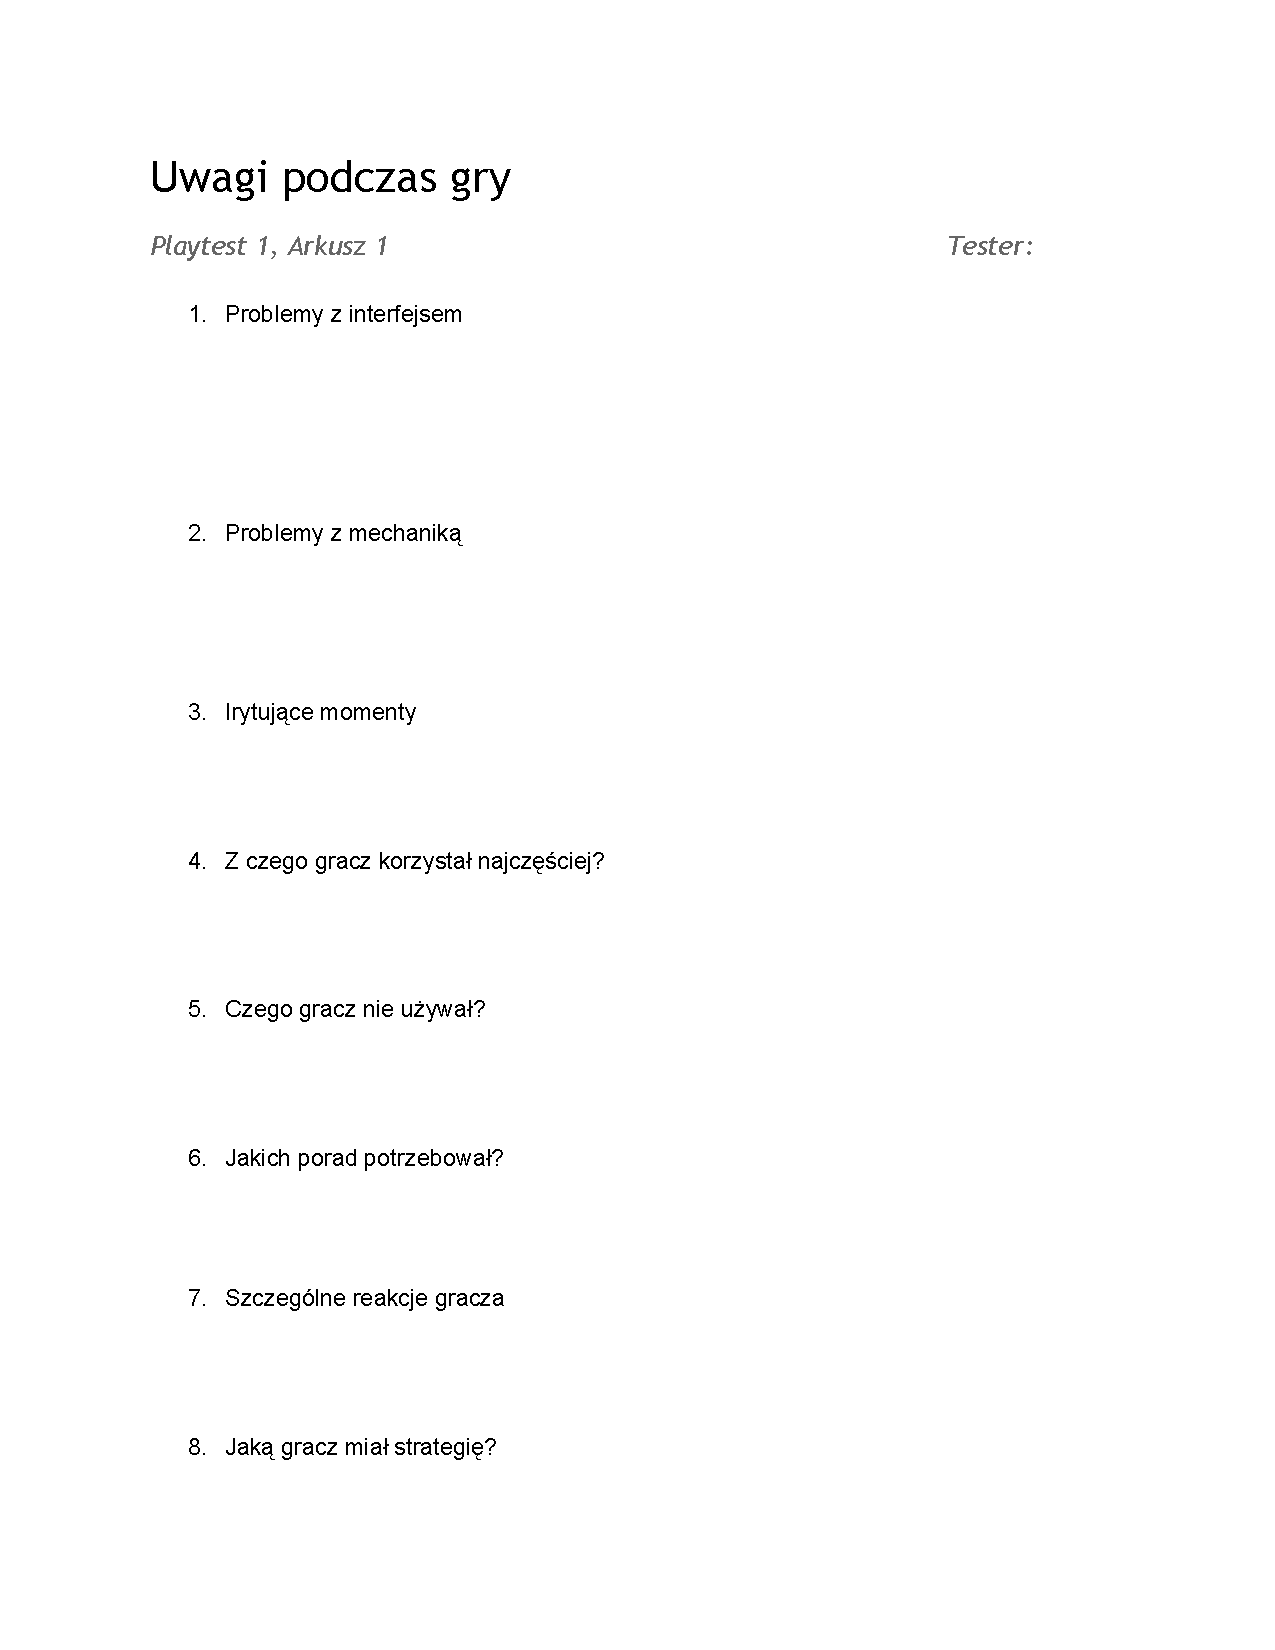
\includepdf[pages={-}]{Formularze-playtesty.pdf}
    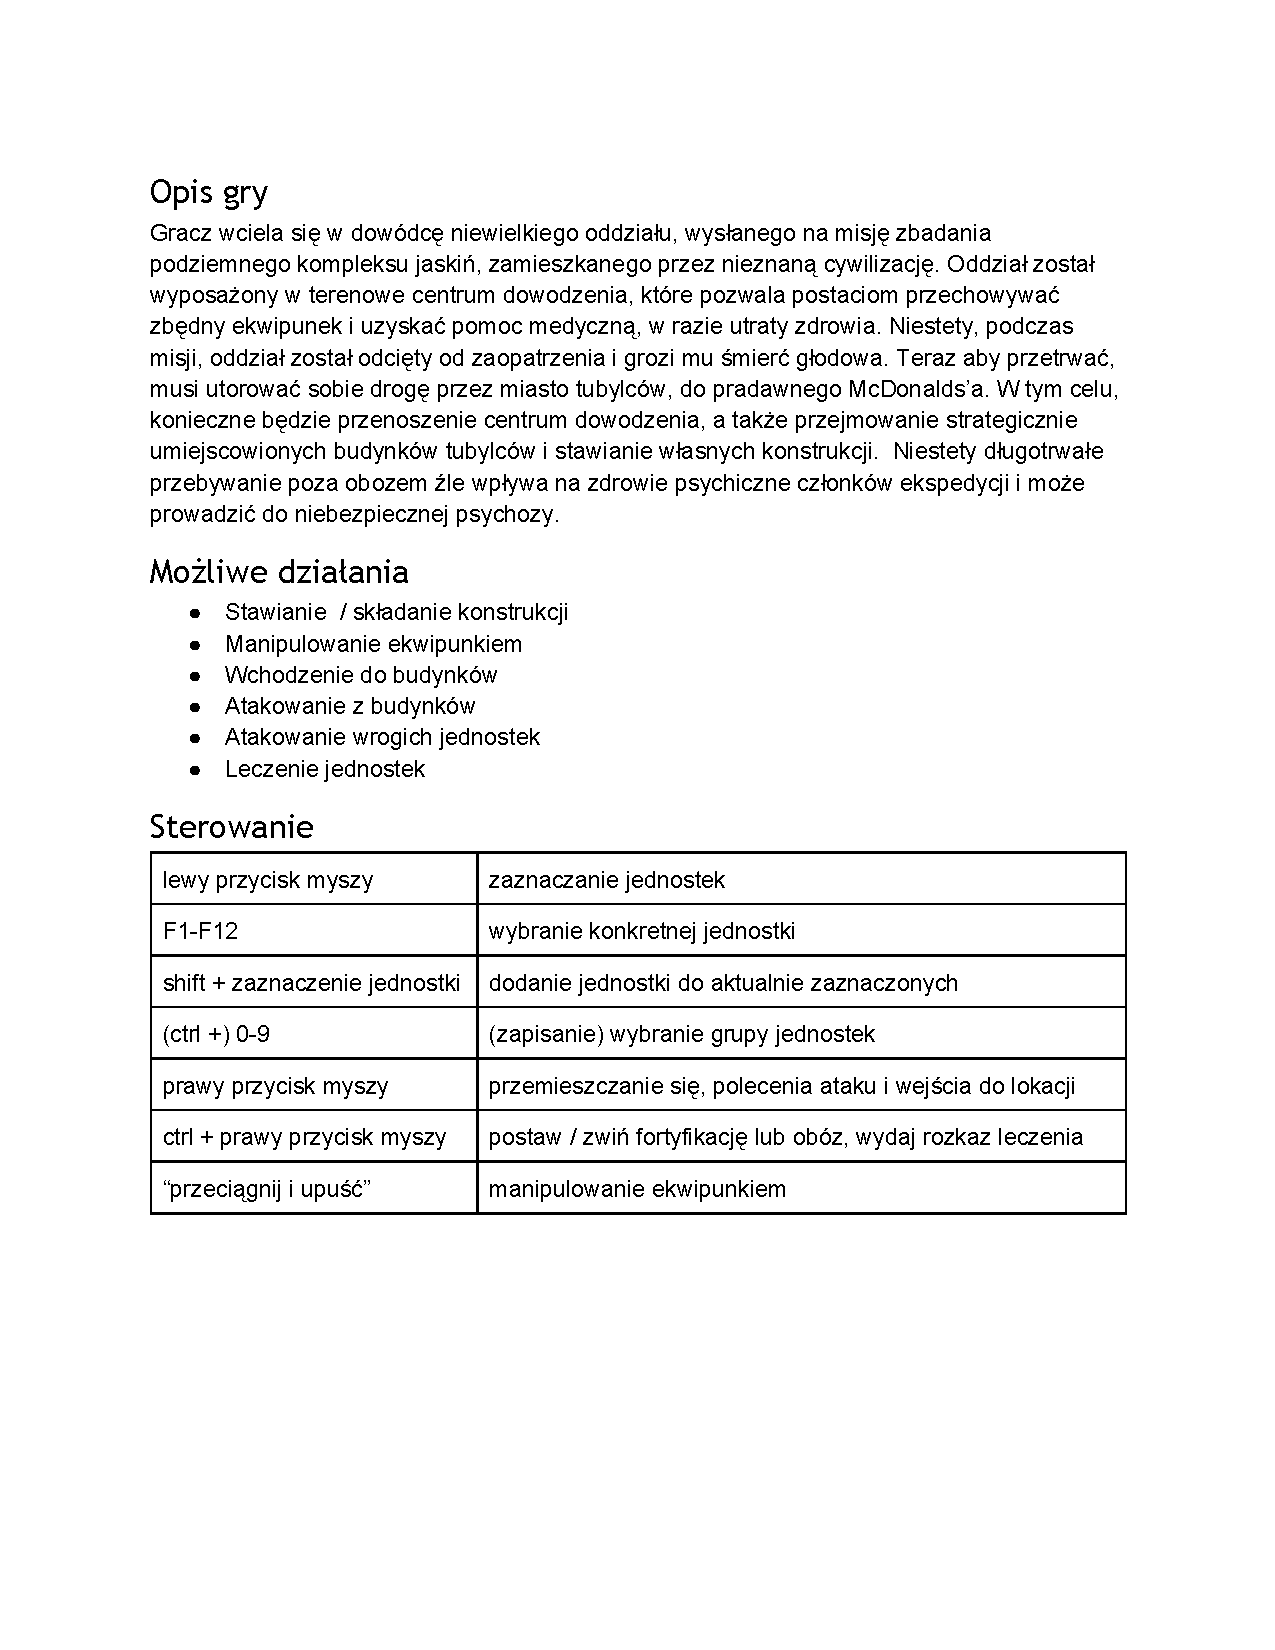
\includepdf[pages={-}]{Instrukcje-do-playtestow.pdf}
    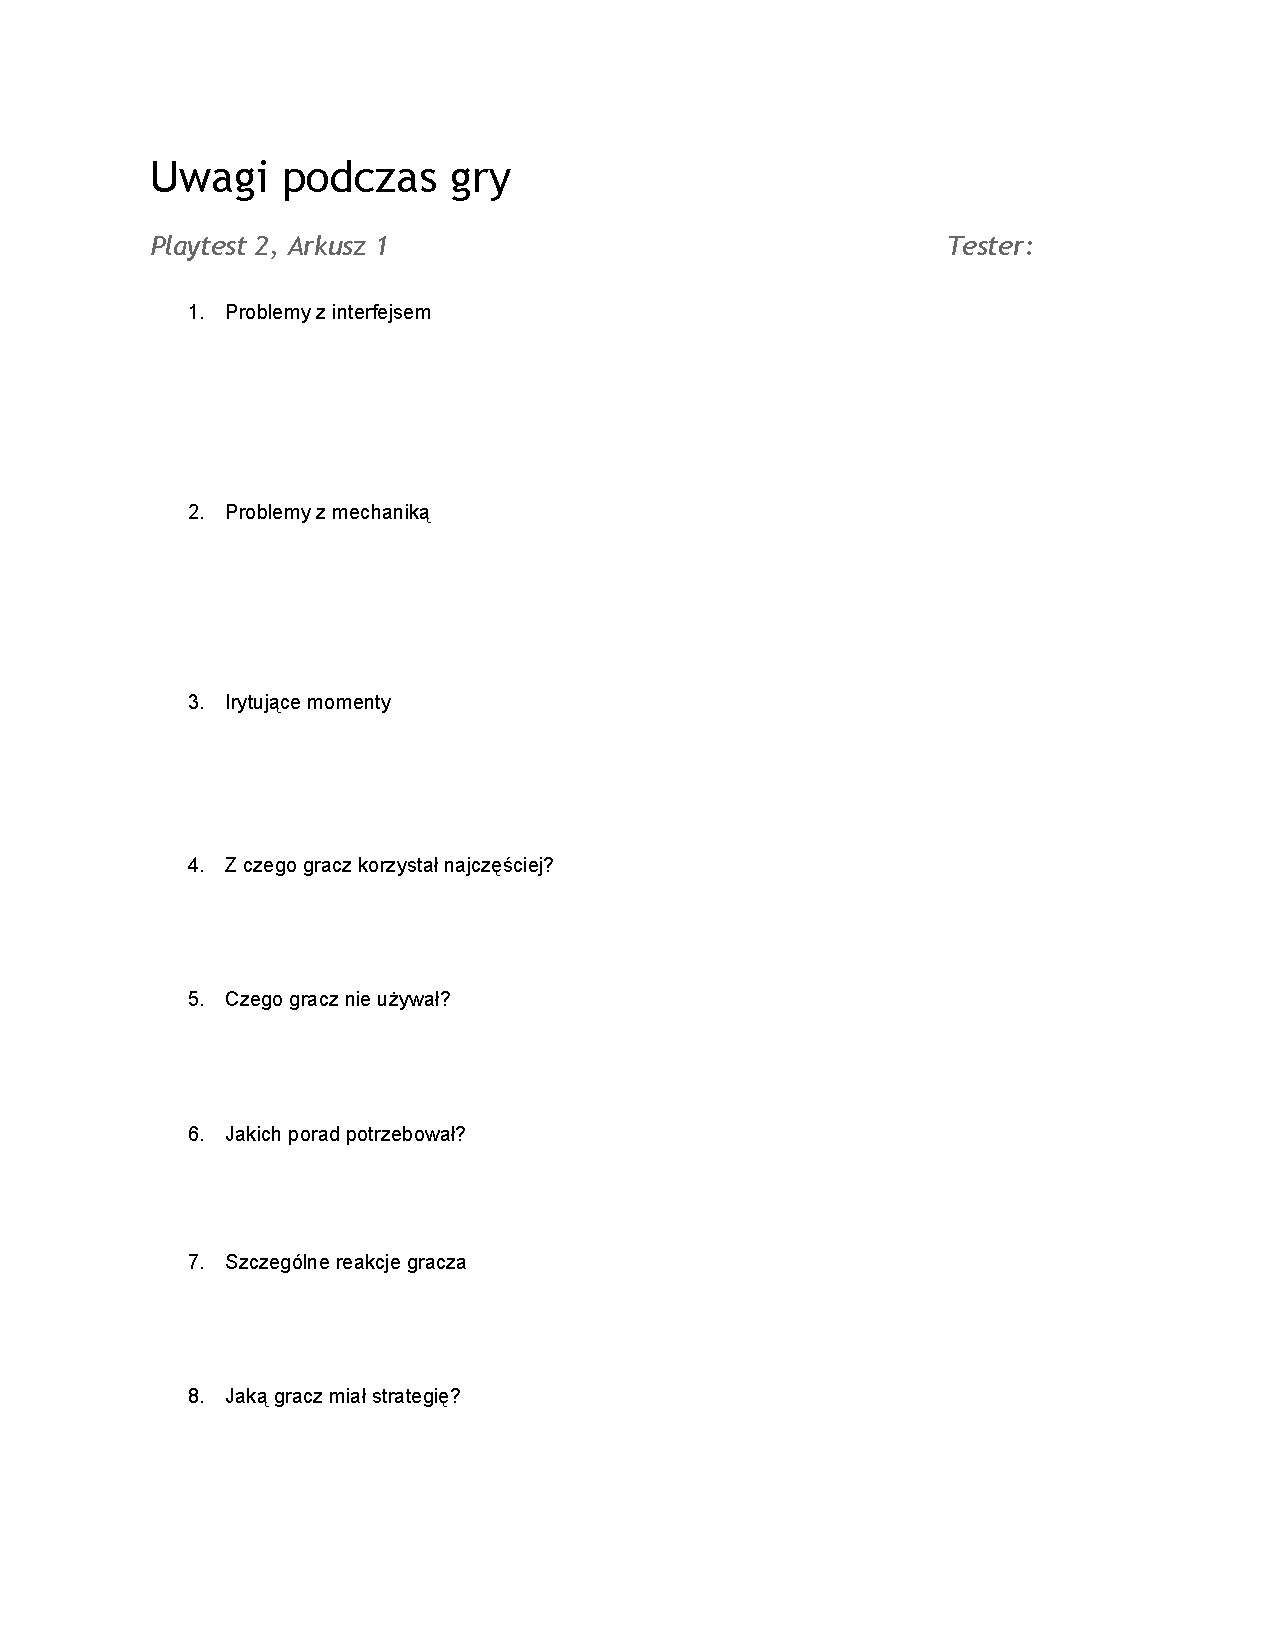
\includepdf[pages={-}]{Formularze-playtesty2.pdf}

  \chapter{Zawarość płyty CD}


\begin{thebibliography}{99}
\addcontentsline{toc}{chapter}{Bibliografia}
  %% To trzeba uładnić
  \item{\url{http://en.wikipedia.org/wiki/Gaussian_blur}}
  \item{Jakiś link z wiki o A*}
  \item{http://webdocs.cs.ualberta.ca/~mmueller/ps/hpastar.pdf - bibliografię pewnie trzeba w ładnym formcie wyciągnąć?}
  \item{\url{http://doc.qt.io/qt-5/reference-overview.html}}

\end{thebibliography}

\end{document}


%%% Local Variables:
%%% mode: latex
%%% TeX-master: t
%%% coding: utf8
%%% End:
